\documentclass[11pt]{article}

\begin{document}
	\begin{appendices}
		\section{Le ray tracer}
			\subsection{Configuration d'une caméra, d'une scène et de rayons}
			\begin{figure}[h!]
				\adjustbox{center}{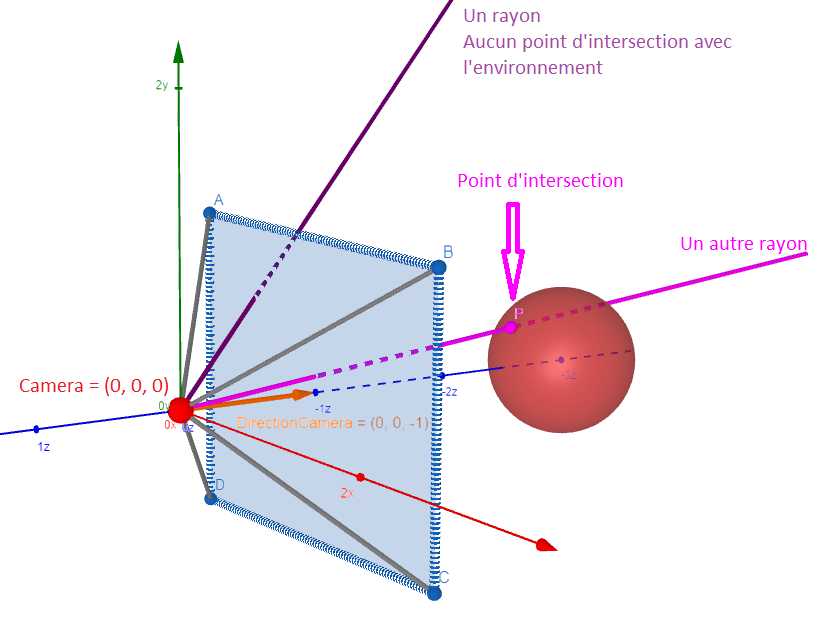
\includegraphics[width=1.1\textwidth]{img/rt/repCam2Rayonsv2.png}}

				\caption{Des rayons sont tirés depuis la caméra dans sa direction de regard. Nous cherchons les points d'intersection avec les objets de la scène.}
			\end{figure}
			\FloatBarrier
			\label{annexe:repreCamRayon}

			\subsection{Le principe récursif des réflexions}
			\begin{figure}[h!]
				\adjustbox{center}{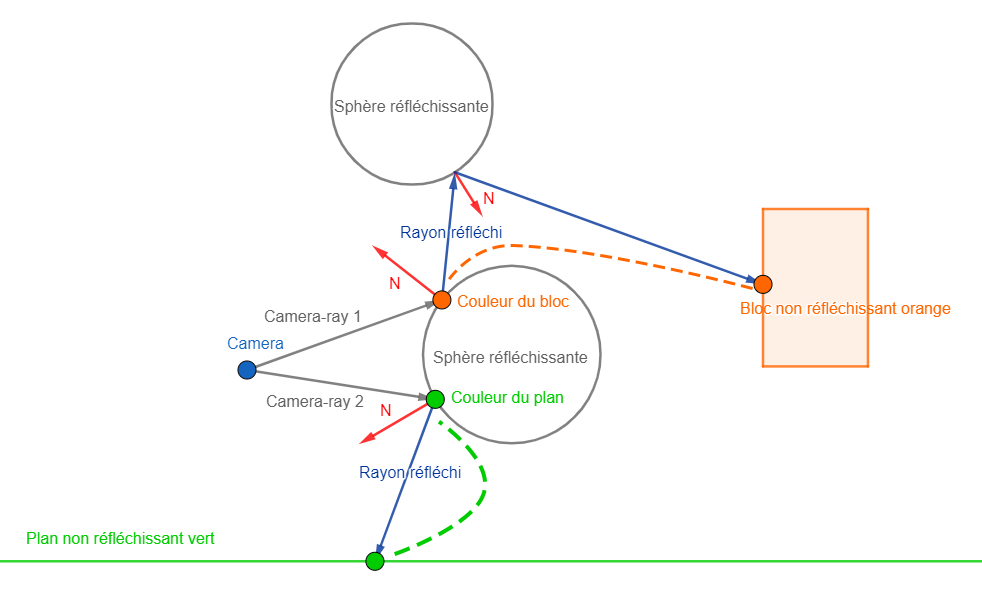
\includegraphics[width=1.1\textwidth]{img/rt/reflectionsSchema.png}}

				\caption{Exemple de rebonds successifs des rayons jusqu'à un objet non réfléchissant}
				\label{reflectionsSchema}
			\end{figure}
			\FloatBarrier
			\label{annexe:reflexionsRecursives}
			
			\subsection{Rotations de la caméra}
			\begin{figure}[h!]
				\adjustbox{center}{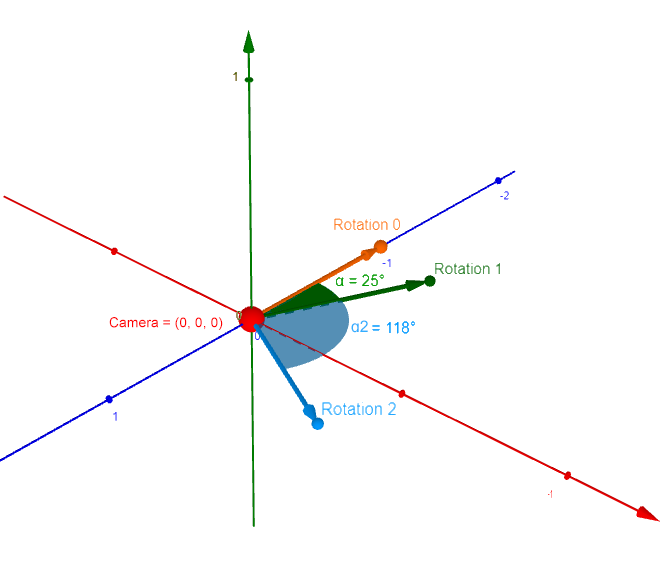
\includegraphics[width = 0.75\textwidth]{img/rt/rotationCameraY.png}}
				
				\caption {Exemples de rotations de la caméra autour de l'axe Y. 'Rotation 0' est la direction de regard de la caméra avant toute rotation.}
			\end{figure}
			\FloatBarrier
			
			\begin{figure}[h!]
				\adjustbox{center}{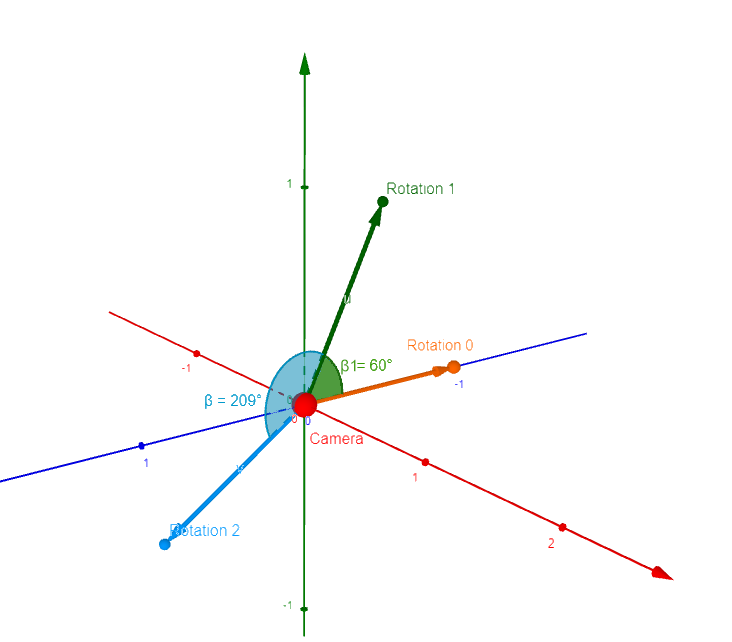
\includegraphics[width = 0.75\textwidth]{img/rt/rotationCameraX.png}}
				
				\caption {Exemples de rotations de la caméra autour de l'axe X. 'Rotation 0' est la direction de regard de la caméra avant toute rotation.}
			\end{figure}
			\FloatBarrier
			\label{annexe:rotationsCamera}
	\FloatBarrier
	\end{appendices}
\end{document}